We now turn to discuss how different predictions compare when the matching to parton-shower (PS) is included. For such
a comparison we expect larger discrepancy than what we found at fixed-order, as a consequence of the different
matching schemes, PS employed and of the other details of the matching (such as the choice of the shower initial scale). Among
the codes capable of providing fixed-order results, presented before, {\sc MG5\_aMC}, {\sc POWHEG} and {\sc VBFNLO}
can also provide results at (N)LO+PS accuracy. For {\sc VBFNLO}, we
restrict ourselves to showing results only in the VBS approximation,
{\emph i.e.} the $s$-channel contributions are neglected here. Besides,
also {\sc PHANTOM} is employed for LO+PS results.\\
{\sc MG5\_aMC},
which
employs the {\sc MC@NLO}~\cite{Frixione:2002ik} matching procedure, will be used together with {\sc Pythia8}~\cite{Sjostrand:2014zea} (version 2.2.3)
and {\sc Herwig++}~\cite{Bahr:2008pv, Bellm:2013hwb} (version 2.7.1). For {\sc POWHEG}, the omonymous matching procedure is
employed~\cite{Nason:2004rx,Frixione:2007vw}, together with {\sc Pythia8}
{\bf MZ VERSION? if same as MG5, put it at the end together with the
tune}. {\sc VBFNLO} serves as a matrix-element and phase-space provider
for the {\sc Matchbox} module~\cite{Platzer:2011bc} of {\sc
Herwig7}~\cite{Bellm:2015jjp,Bellm:2017bvx}, using an extended version of the BLHA
interface~\cite{Binoth:2010xt,Alioli:2013nda,Andersen:2014efa}. The {\sc Matchbox} module makes it
possible to choose between {\sc MC@NLO}-like and {\sc POWHEG}-like
matching. As parton shower, both the default angular-ordered shower as
well as the dipole shower can be employed.
Finally, {\sc PHANTOM} results will be shown matched with {\sc Pythia 8} and {\sc Herwig++}.
Whenever {\sc Pythia8}\ is used, the Monash tune~\cite{Skands:2014pea} is selected.\\

Results will be presented within the cuts described in Section~\ref{subsec:inputpar}, applied after shower and hadronization (this implies that jets
are obtained by clustering stable hadrons, and not QCD partons). It follows that at the event-generation level, looser cuts (or no cuts at all)
must be employed in order not to bias the results. {\bf MZ lepton-jet separation at the hard-event level?}.\\

A slightly different setup has been employed for {\sc MG5\_aMC} in order to simplify the calculation: instead of generating the full
${\rm p}{\rm p}\to\mu^+\nu_\mu{\rm e}^+\nu_{\rm e}{\rm j}{\rm j}$ process, since it is anyway dominated by doubly-resonant contribution, the
events are produced for the process with two stable W$^+$ bosons (${\rm p}{\rm p}\to{\rm W^+}{\rm W^+}{\rm j}{\rm j}$), and these W$^+$ bosons
are decayed with {\sc MadSpin}~\cite{Artoisenet:2012st} (keeping spin correlations) before the PS. Since {\sc MadSpin}\ computes
the partial and total decay width of the W bosons at LO accuracy only, while in Section~\ref{subsec:inputpar} the NLO width is employed,
a small effect (6\%) on the normalisation of distribution is induced. Finally, when the renormalisation
and factorisation scales are set, the $\Delta R_{\Pj\Pl}$ cut is not imposed during the jet-clustering procedure, but this has no visible effect
on the results.

\begin{table}[h!]
    \centering
    \begin{tabular}{c|r@{ $\pm$ }l}
      Code  &  \multicolumn{2}{c}{$\sigma[\rm{fb}]$}  \\
        \hline\hline
        {\sc MG5\_aMC}+{\sc Pythia8}&  $1.450 (1.368)$ & $0.004$  \\
        {\sc MG5\_aMC}+{\sc Herwig++}&  $1.445 (1.363)$ & $0.004$  \\
        {\sc POWHEG}  &  $1.3642$ & $0.0004$  \\
        {\sc VBFNLO}+{\sc Herwig7-Dipole} &  $1.3389$ & $0.0006$  \\
        {\sc VBFNLO}+{\sc Herwig7-Default} &  $1.3067$ & $0.0006$  \\
        \hline
        {\sc MG5\_aMC}+{\sc Pythia8} (LO)&  $1.352 (1.275)$ & $0.003$  \\
        {\sc MG5\_aMC}+{\sc Herwig++} (LO)&  $1.343 (1.267)$ & $ 0.003$  \\
        {\sc PHANTOM}+{\sc Pythia8} &  $1.235\phantom{0} $ & $0.001$  \\
        {\sc PHANTOM}+{\sc Herwig++} &  $1.260\phantom{0} $ & $0.001$  \\
        {\sc VBFNLO}+{\sc Herwig7} (LO) &  $1.3001$ & $0.0002$  \\
    \end{tabular}
    \caption{\label{tab:PSrates} Rates at NLO-QCD (LO-QCD) accuracy matched to parton shower within VBS cuts obtained with the different codes used in this comparison,
    for the ${\rm p}{\rm p}\to\mu^+\nu_\mu{\rm e}^+\nu_{\rm e}{\rm j}{\rm j}$ process. Numbers in parentheses for the {\sc MG5\_aMC} simulations
    are rescaled to account for the effect related to the boson widths computed by {\sc MadSpin}, see the text for details.}
\end{table}

We now turn to present the results of predictions matched to parton shower: the total rates within VBS cuts are displayed in Table~\ref{tab:PSrates}, both at LO and NLO
accuracy. For {\sc MG5\_aMC}, the numbers in parentheses are rescaled to take into account the width effects described in the above paragraph. Once this effect is taken into
account, total rates from different tools agree within few percents. Larger discrepancies however will appear for differential observables, which we are going to discuss in
the following. For any observable, results will be presented in two plots, shown side-by-side. In the plot on the left (right), (N)LO+PS predictions are shown
with different colours in the main frame. In the inset, these predictions are compared in both cases with the fixed-order prediciton at NLO accuracy (obtained with
{\sc VBFNLO}). For the differential observables, the {\sc MG5\_aMC} predictions are \emph{not} rescaled to compensate for the width effect mentioned above.\\

The first observable we investigate is the exclusive jet multiplicity, shown in Figure~\ref{fig:PSnjet}. Looking at the LO+PS predictions, one can appreciate that the
main effects are driven by the parton shower that is employed {\sc Herwig++/7} or {\sc Pythia8}, with the clear tendency of producing more radiation for the latter,
leading to higher jet multiplicities. Difference among tools that employ the same parton shower are typically smaller, and can be traced back to different values of the
initial scale of the shower. The main effect of NLO corrections for this (rather inclusive) observable is to stabilize the predictions for the two-jet bin, where discrepancies
among tools are reduced to about 10\%. For the three-jet bin, which is described only at LO accuracy, differences among tools remain large: the largest rate is predicted by
{\sc MG5\_aMC}, while the smallest rate is predicted by {\sc Powheg}, both matched to {\sc Pythia8}. Despite the fact that the same parton shower is employed, the way emissions are treated
is different among the two tools. In particular, for {\sc Powheg}, the first emission is generated with an internal Sudakov form factor (the
prediction dubbed {\sc Powheg-no shower} corresponds to stopping after the first emission), while for {\sc MG5\_aMC} there is an
interplay between the real-emission matrix element and the shower emission. \\
The next observable that we study is the invariant mass of the two tagging jets, shown in Figure~\ref{fig:PSmjj}. For this observable, both at LO+PS and NLO+PS,
the spread of predictions matched with parton shower is rather small
($\lesssim 10\%$, if one compensates for the 6\% width effect for {\sc MG5\_aMC}); LO+PS predictions tend to be significantly softer than the fixed NLO one, with an effect of
about -30\% at the end of the displayed range. At NLO+PS, this effect is much mitigated, owing to the better description of the first QCD emission which is now driven by
 the real-emission matrix element.\\
The rapidity difference between the two tagging jets, shown in Figure~\ref{fig:PSdyjj} has some similarities to the invariant-mass distribution: at LO+PS all predictions,
except for {\sc VBFNLO3+Herwig7} where the effect is mitigated, show the tendency to deplete the large-separation region with respect to the fixed-order predicion, in a
quantitatively similar way. At NLO+PS, when the extra radiation is described by the real matrix element, such an effect is greatly reduced. A notable
exception is the {\sc Powheg} prediction, which still shows a suppression at large separations: since such a suppression is already there for the {\sc Powheg-no shower} sample,
it is very likely that it is driven by the way the first emission is generated. A minor effect in the same direction is visible in the last two bins of the
{\sc MG5\_aMC+Herwig++} prediction (although with rather large statistical uncertainties).\\
The transverse momentum of the hardest and second-hardest jets are shown in Figures~\ref{fig:PSpt1} and~\ref{fig:PSpt2} respectively. In general, for both observables,
predictions from different tools agree rather well with each other, with a spread at most at the 10\% level. At LO+PS, typically the transvers-momentum spectra are softer than
the fixed-NLO one, and this effect is more marked for the second-hardest jet which, as expected, is more sensitive to the description of the extra radiation. Again, this
effect is mitigated by NLO corrections. The only feature that it may be worth to notice among the NLO+PS predictions is the tendency of {\sc Powheg} to suppress the
hardest-jet spectrum at low transverse momentum ($p_T<100 \GeV$).\\
If we consider the rapidity of the second jet, Figure~\ref{fig:PSy2}, we observe again rather small differences among tools, with the tendency towards a general
stabilization at NLO+PS. However, some (small) differences in the shape remain at NLO+PS, which are worth to be briefly discussed: predictions
obtained with {\sc MG5\_aMC} are very close to the fixed-order prediction; {\sc Powheg}\ displays an enhancement of the central region, and a consequent suppression in the
peripheral region, while {\sc VBFNLO} shows an opposite behaviour. However, the effect is rather small, with the largest departure from the fixed-order prediction being
at most 10\%.\\
Finally, focusing on the third jet, we conclude the list of differential observables with the rapidity and the Zeppenfeld variable defined in Eq.~\eqref{eq:Zeppenfeld}, Figures~\ref{fig:PSy3} and~\ref{fig:PSz3}.
{\bf MZ the rapidity can be dropped (check also the following discussion in case); if z is defined elsewhere in the paper, then add a ref to the proper section. Otherwise define it here}
In general, for observables which involve the third jet, one
can clearly see a degradation of the agreement among the various tools, because of the poorer perturbative description of these observables. The rapidity and $z$ variable
are a striking example: both at LO and NLO, the tendency of {\sc Pythia8} to generate more hard and central radiation (corresponding to low values of $z$)
is clearly visible; it is interesting to notice that
this effect survives beyond the first emission, as it can be observed by comparing {\sc Powheg-no shower} with {\sc Powheg+Pythia8}. If it is true that the central enhancement
is a bit mitigated if NLO+PS tools are used (compare LO+PS and NLO+PS from {\sc MG5\_aMC+Pythia8} with the fixed-NLO prediciton), however even at NLO+PS the central region
($z_{j_3}<0.5$) is cursed by huge differences between tools. Large differences, reaching a factor 2, persist also away from the central region. \\

In conclusion, the comparison of tools including matching with parton-shower clearly shows the benefits of the inclusion of NLO corrections: for most observables described
effectively at NLO accuracy differences between tools are at (or below) the 10\% level. {\bf MZ compare this number with scale uncertainties}
Some exceptions exist, e.g. the rapidity separation of the two tagging jets, which
on the one hand clearly suggest not to rely on a single tool/parton shower, and on the other make it worth to investigate more in details the way QCD radiation is
generated {\bf MZ cite here H VBF at NNLO?}. Finally, the size of discrepancies for observables that are described at a lower perturbative accuracy, notably those related to the third jet, suggest that
experimental analyses should rely as least as possible on those observables and, in any case, use conservative estimate of the theory uncertainties. In order to improve the
description of these observables, a simulation of VBS+j at NLO, currently unavailable but within the reach of modern automated tools, is certainly desirable.

\begin{figure*}[hbt]
\centering
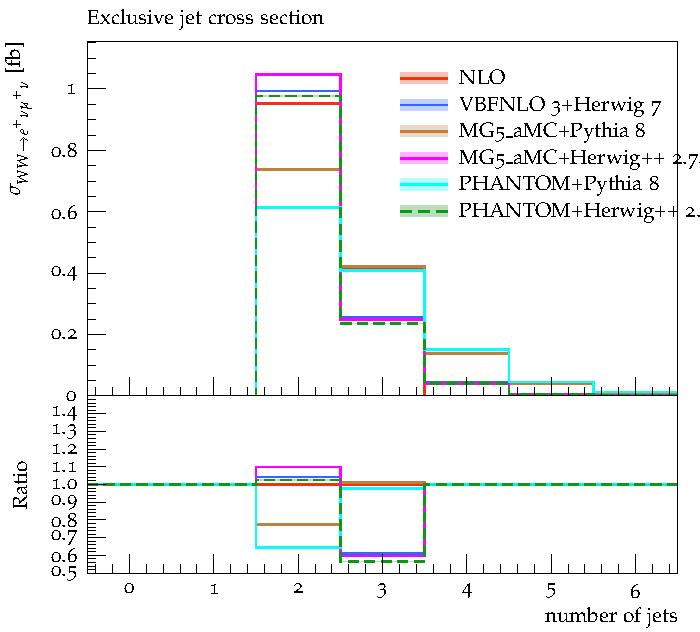
\includegraphics[width=0.47\textwidth]{figures/LOPS/jetsexclusive.pdf}
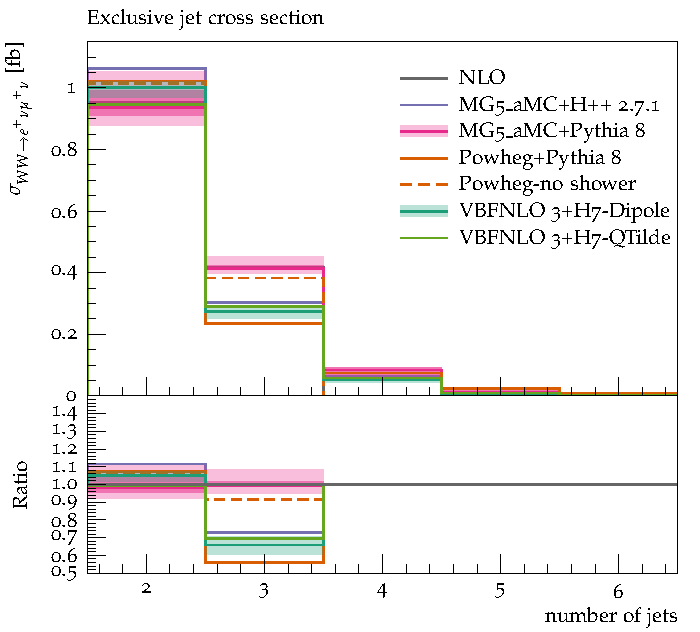
\includegraphics[width=0.47\textwidth]{figures/NLOPS/jetsexclusive.pdf}
\caption{Exclusive jet multiplicity from predictions matched to parton shower, at LO (left) or NLO (right) accuracy, compared with the fixed-NLO result
    computed with \sc{VBFNLO}}
\label{fig:PSnjet}
\end{figure*}

\begin{figure*}[hbt]
\centering
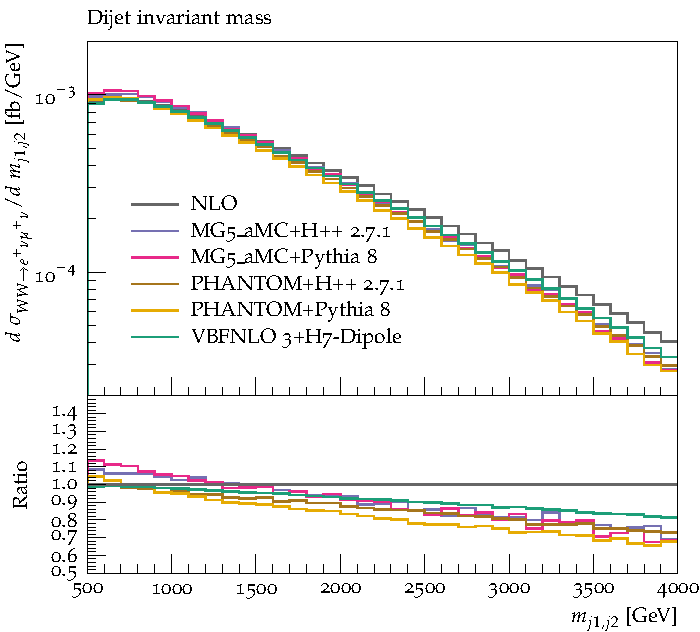
\includegraphics[width=0.47\textwidth]{figures/LOPS/m_jj.pdf}
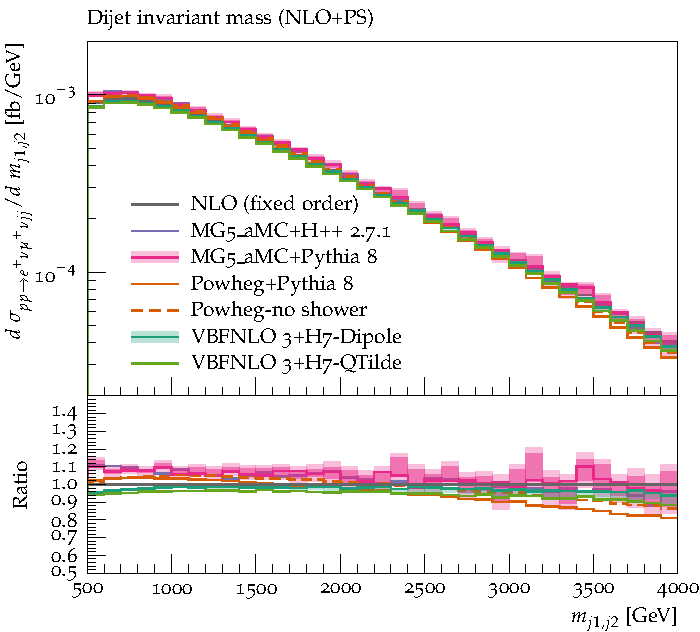
\includegraphics[width=0.47\textwidth]{figures/NLOPS/m_jj.pdf}
\caption{Same as in Fig.~\protect\ref{fig:PSnjet}, for the invariant mass of the two tagging jets.}
\label{fig:PSmjj}
\end{figure*}

\begin{figure*}[hbt]
\centering
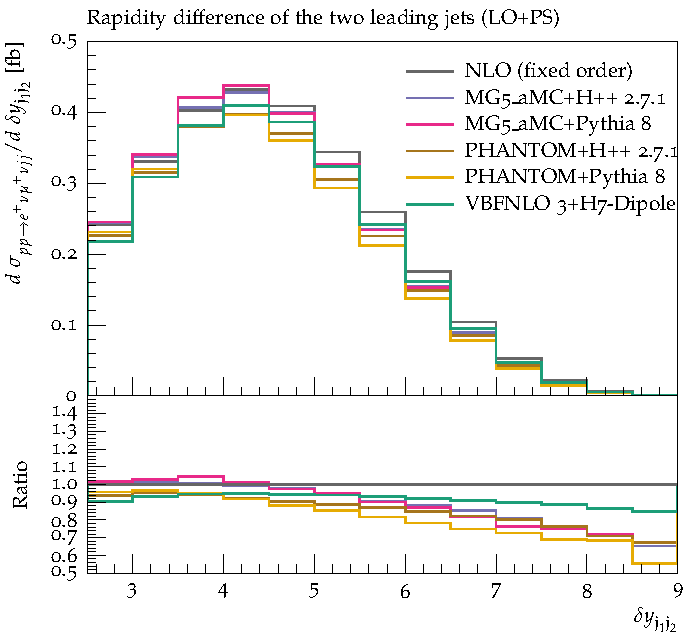
\includegraphics[width=0.47\textwidth]{figures/LOPS/Deltay_jj.pdf}
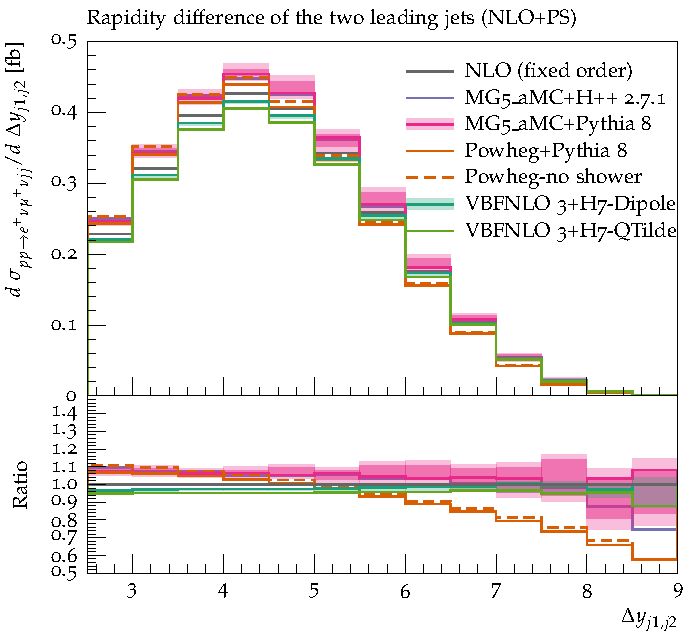
\includegraphics[width=0.47\textwidth]{figures/NLOPS/Deltay_jj.pdf}
\caption{Same as in Fig.~\protect\ref{fig:PSnjet}, for the rapidity separation of the two tagging jets.}
\label{fig:PSdyjj}
\end{figure*}

\begin{figure*}[hbt]
\centering
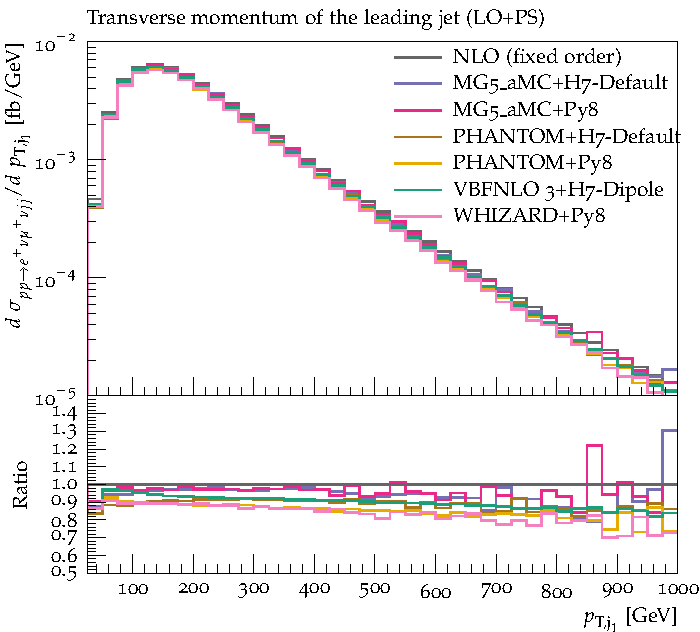
\includegraphics[width=0.47\textwidth]{figures/LOPS/pT_j1.pdf}
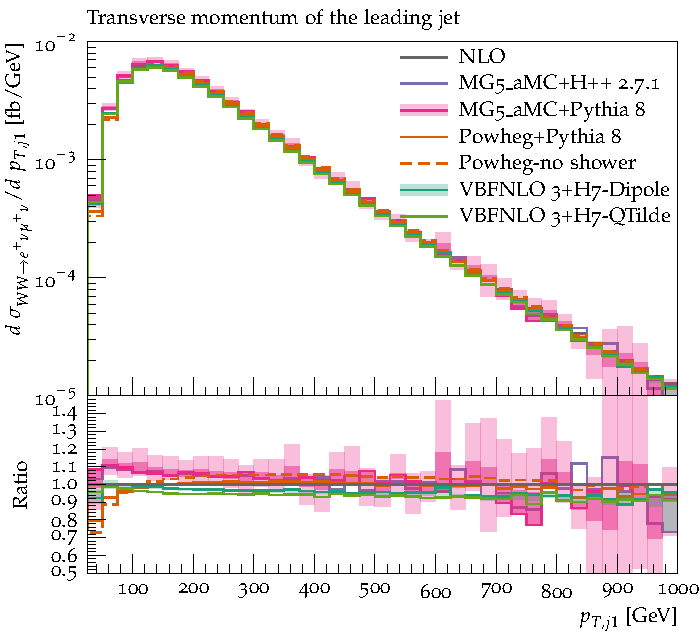
\includegraphics[width=0.47\textwidth]{figures/NLOPS/pT_j1.pdf}
\caption{Same as in Fig.~\protect\ref{fig:PSnjet}, for the transverse momentum of the hardest jet.}
\label{fig:PSpt1}
\end{figure*}

\begin{figure*}[hbt]
\centering
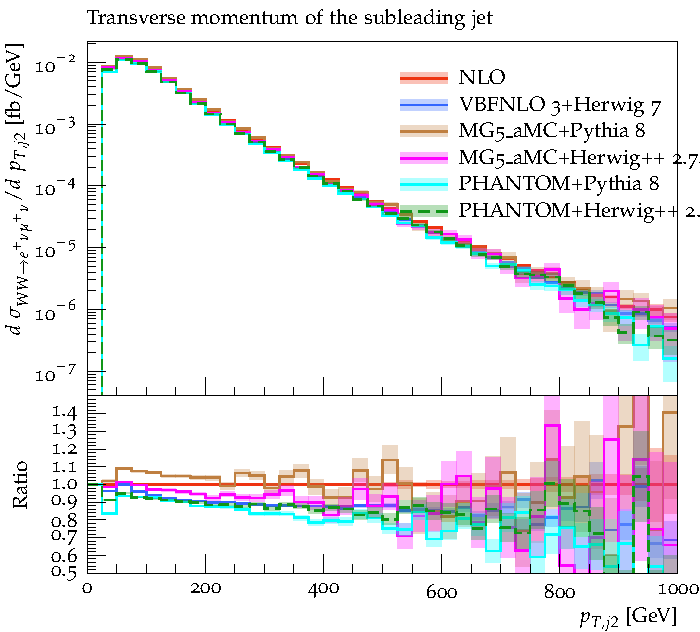
\includegraphics[width=0.47\textwidth]{figures/LOPS/pT_j2.pdf}
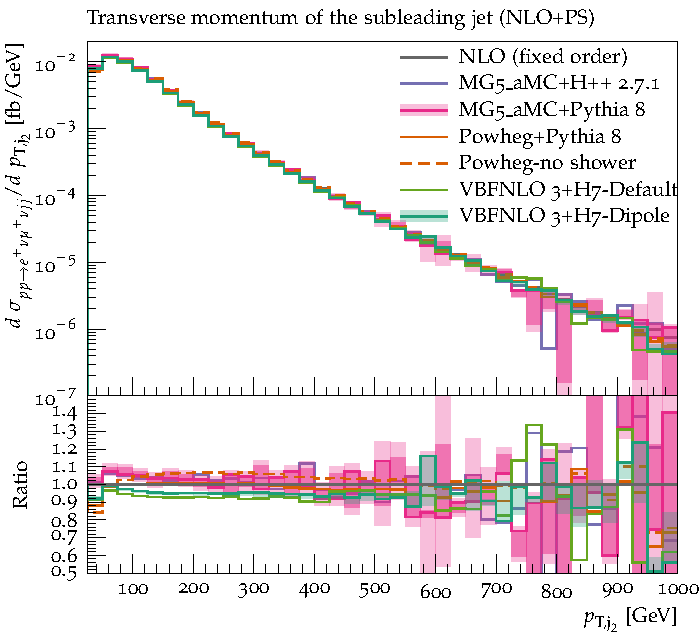
\includegraphics[width=0.47\textwidth]{figures/NLOPS/pT_j2.pdf}
\caption{Same as in Fig.~\protect\ref{fig:PSnjet}, for the transverse momentum of the second-hardest jet.}
\label{fig:PSpt2}
\end{figure*}

\begin{figure*}[hbt]
\centering
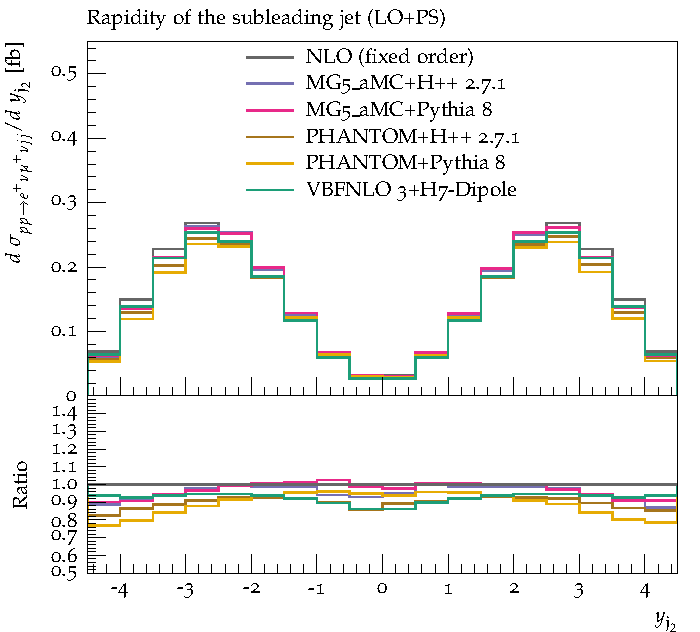
\includegraphics[width=0.47\textwidth]{figures/LOPS/y_j2.pdf}
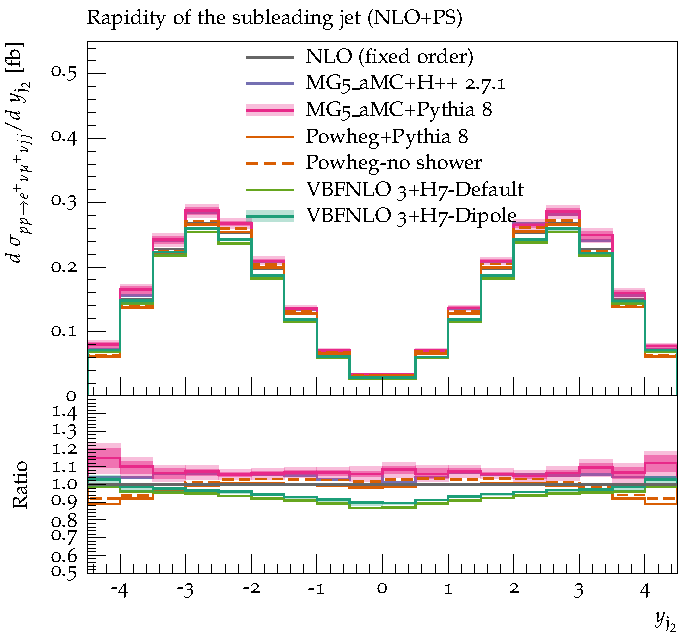
\includegraphics[width=0.47\textwidth]{figures/NLOPS/y_j2.pdf}
\caption{Same as in Fig.~\protect\ref{fig:PSnjet}, for the rapidity of the second-hardest jet.}
\label{fig:PSy2}
\end{figure*}

\begin{figure*}[hbt]
\centering
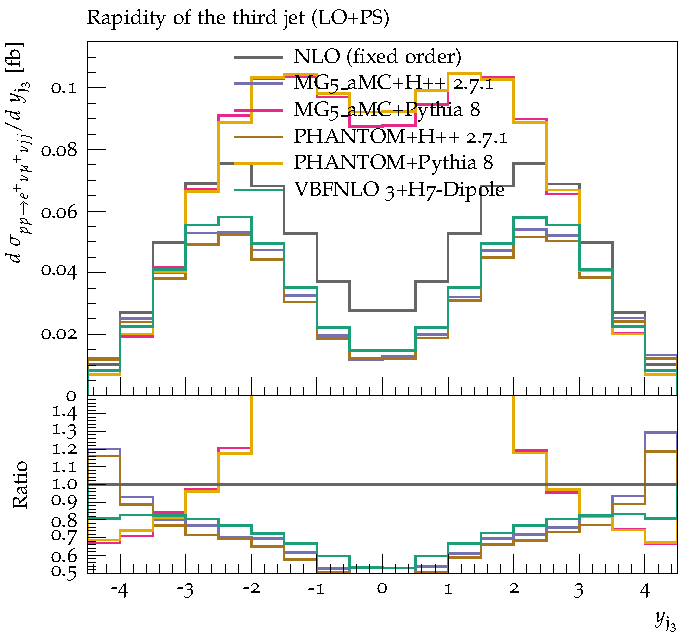
\includegraphics[width=0.47\textwidth]{figures/LOPS/y_j3.pdf}
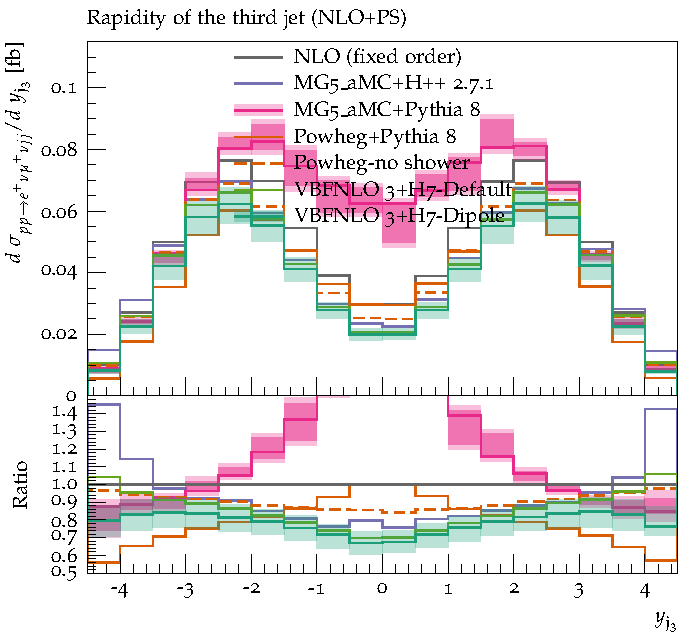
\includegraphics[width=0.47\textwidth]{figures/NLOPS/y_j3.pdf}
\caption{Same as in Fig.~\protect\ref{fig:PSnjet}, for the rapidity of the third-hardest jet.}
\label{fig:PSy3}
\end{figure*}

\begin{figure*}[hbt]
\centering
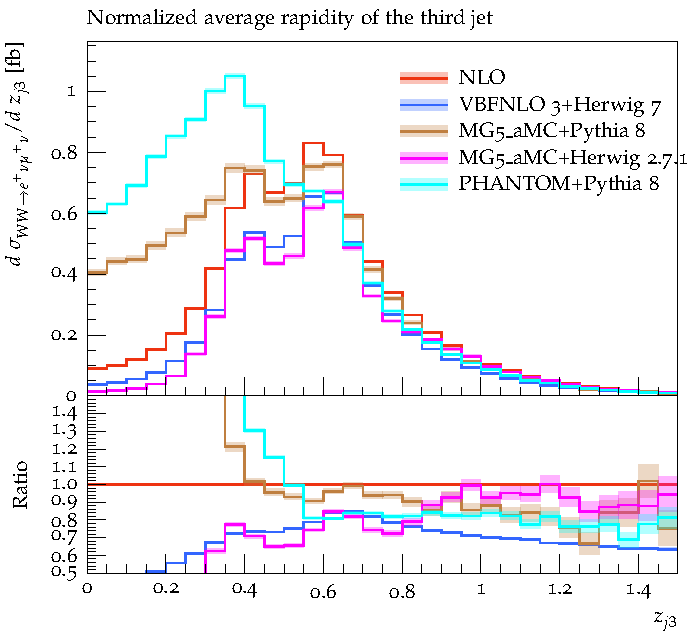
\includegraphics[width=0.47\textwidth]{figures/LOPS/z_j3.pdf}
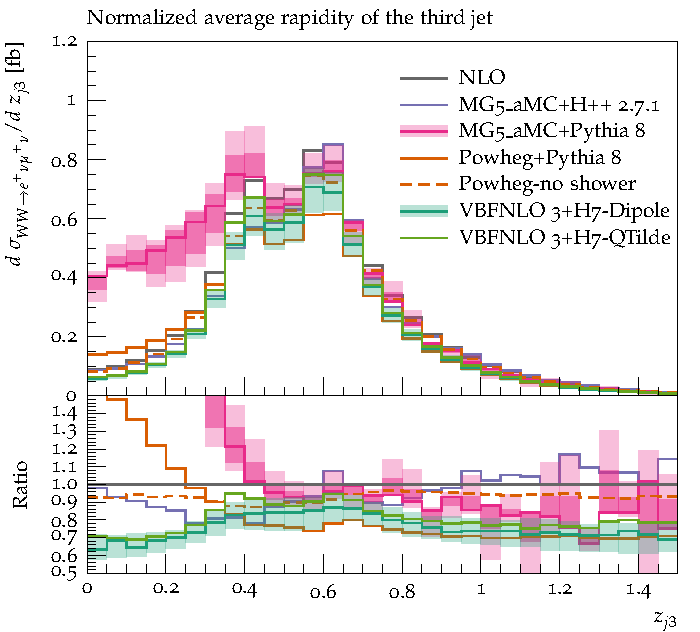
\includegraphics[width=0.47\textwidth]{figures/NLOPS/z_j3.pdf}
\caption{Same as in Fig.~\protect\ref{fig:PSnjet}, for the $z$ variable of the third-hardest jet.}
\label{fig:PSz3}
\end{figure*}
